

\documentclass{beamer}

\usepackage{graphicx}

\usepackage[a4paper, total={6in, 8in}]{geometry}
% tikz package is required to use TikZ in LaTeX document.
\usepackage{tikz}
% \usetheme{default}
% shapes.geometric is a TikZ library defining basic geometric objects.
\usetikzlibrary{shapes.geometric}

\usepackage{amsmath}
\usetheme{Madrid}


\title{Fast Fourier Transform}
\subtitle{Revolutionizing algorithm}
\author[Turad \and Tanvir \and Jakaria]
{Md. Tanvirul Islam Turad (2005011)\\
Tanvir Hossain (2005014)\\
Md. Jakaria Hossain (2005026)\\}
\institute[CSE, BUET]
{
	Department of CSE\\
	Bangladesh University of Engineering and Technology
}
\date{\today}

\AtBeginSection
{
	\begin{frame}
		\frametitle{Table of Contents}
		\tableofcontents[currentsection]
	\end{frame}
}

\begin{document}
	
	\frame{\titlepage}
	
%	\begin{frame}
%		\frametitle{Table of Contents}
%		\tableofcontents
%	\end{frame}
	
	

%             \begin{frame}{Motivation}
%   \begin{itemize}
%     \item Analyze signals in the frequency domain to understand their composition.
%     \item Limitations of the Discrete Fourier Transform (DFT):
%       \begin{itemize}
%         \item Quadratic time complexity  $(O(N^2))$, computationally expensive for large signals.
%         \item Need for a faster and more efficient algorithm.
%       \end{itemize}
%     \item Applications:
%       \begin{itemize}
%         \item Signal processing (noise removal, filtering,...)
%         \item Image processing (compression, feature extraction,...)
%         \item Speech and audio processing (compression, synthesis,...)
%         \item Scientific computing (solving differential equations, analyzing time-series data)
%       \end{itemize}
%   \end{itemize}
% \end{frame}
\begin{frame}{Introduction to FFT}
  \begin{itemize}
    \item The Fast Fourier Transform (FFT) is an algorithm to compute the Discrete Fourier Transform (DFT) and its inverse.
    \item It drastically reduces the computational complexity of computing DFT, making it feasible for real-time processing.
    \item Developed by Cooley and Tukey in 1965, FFT has become a fundamental tool in various fields such as signal processing, image processing, and more.
    \item This presentation aims to provide an overview of FFT, its significance, and applications.
  \end{itemize}
\end{frame}

\section{Background}
\begin{frame}{Fourier Transform}
  \begin{itemize}
    \item Fourier Transform decomposes a signal into its frequency components.
    \item It represents a signal in terms of sinusoidal basis functions.
    \item The continuous Fourier Transform is given by:
    \[ F(\omega) = \int_{-\infty}^{\infty} f(t) e^{-i\omega t} dt \]
    where $f(t)$ is the signal, and $F(\omega)$ is its frequency domain representation.
  \end{itemize}
\end{frame}

\begin{frame}{Discrete Fourier Transform (DFT)}
  \begin{itemize}
    \item DFT is the discrete counterpart of the continuous Fourier Transform.
    \item It is defined as:
    \[ X[k] = \sum_{n=0}^{N-1} x[n] e^{-i2\pi kn/N} \]
    where $x[n]$ is the discrete signal, and $X[k]$ is its frequency domain representation.
    \item Direct computation of DFT is of $O(N^2)$ complexity.
  \end{itemize}
\end{frame}

\section{Motivation}
 
            \frame{
              \frametitle{Motivation}
              \begin{itemize}
                \item Analyze signals in the frequency domain to understand their composition.
                \item Limitations of the Discrete Fourier Transform (DFT):
                  \begin{itemize}
                    \item Quadratic time complexity $$O(N^2)$$ computationally expensive for large signals.
                    \item Need for a faster and more efficient algorithm.
                  \end{itemize}
                \item Applications:
                  \begin{itemize}
                    \item Signal processing (noise removal, filtering,...)
                    \item Image processing (compression, feature extraction,...)
                    \item Speech and audio processing (compression, synthesis,...)
                    \item Scientific computing (solving differential equations, analyzing time-series data)
                  \end{itemize}
              \end{itemize}
            }

\section{The Fast Fourier Transform (FFT)}
\begin{frame}{The Fast Fourier Transform (FFT)}
  \begin{itemize}
    \item FFT is an efficient algorithm for computing DFT.
    \item It exploits the periodicity and symmetry properties of sinusoidal functions to reduce the number of computations.
    \item The Cooley-Tukey algorithm is the most popular FFT algorithm.
    \item It divides the DFT computation into smaller DFTs, recursively applies FFT, and combines the results to obtain the final DFT.
    \item FFT reduces the computational complexity to $O(N\log N)$, making it feasible for real-time applications.
  \end{itemize}
\end{frame}

	\section{Polynomial Representation}

\begin{frame}{An Optimization Problem}
    \pause
    Let's multiply two quadratic polynomials:
    \pause
    \begin{equation*}
        \begin{split}
            P(x) & = (a_0 + a_1x + a_2x^2) \times (b_0 + b_1x + b_2x^2) \\
                 & = c_0 + c_1x + c_2x^2 + c_3x^3 + c_4x^4
        \end{split}
    \end{equation*}
    \pause
    \begin{equation*}
        \begin{split}
            c_0 & = a_0b_0                   \\
            c_1 & = a_0b_1 + a_1b_0          \\
            c_2 & = a_0b_2 + a_1b_1 + a_2b_0 \\
            c_3 & = a_1b_2 + a_2b_1          \\
            c_4 & = a_2b_2
        \end{split}
    \end{equation*}

        $$O(n^2) $$
    \pause
    \text{Can we do better?}
\end{frame}
 
		\begin{frame}{Polynomial Representation}
                \centering
              
              Two Unique Representation for Polynomials: 
              \begin{equation*}
                  P(x) = p_0 + p_1x + p_1x^2 + ... + p_dx^d
              \end{equation*}
              \begin{itemize}
                  \item Coefficient Representation: 
                    \begin{equation*}
                        [p_0, p_1, p_2,... p_d]
                    \end{equation*}
                    \item Value Representation: 
                    \begin{equation*}
                        [(x_0, P(x_0)), (x_1, P(x_1)), ... (x_d, P(x_d))]  
                    \end{equation*}
              \end{itemize}
                
                
		\end{frame}

	    \begin{frame}{Why Value Representation}

                        \begin{columns}
        				\column[]{0.5\textwidth}
        	               \begin{equation*}
                                    A(x) = x^2 + 2x +1
        	               \end{equation*}			
                         \small  {[(-2, 1), (-1, 0), (0,1), (1,4), (2, 9)]}
        				\column[]{0.5\textwidth}
                              \begin{equation*}
        				        B(x) = x^2 - 2x + 1
                                \end{equation*}
                         \small  {[(-2, 9), (-1,4), (0,1), (1,0), (2, 1)]}
                                
                            
        			 \end{columns}

% figure
            
             \vspace{0.5cm} 
                            \begin{equation*}
                                C(x) = A(x).B(x)
                            \end{equation*}
                    \centering
                         \small  {(-2, 1), (-1, 0), (0,1), (1,4), (2, 9)}\\
                       x  \small  {(-2, 9), (-1,4), (0,1), (1,0), (2, 1)}\\

                         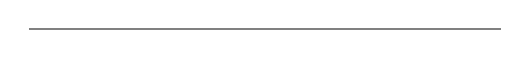
\begin{tikzpicture}
                            \draw[gray, thick] (-3, 0) -- (3, 0);  % Straight Line
                        \end{tikzpicture}
                        \\
                     C(x) =\small  {(-2, 9), (-1,0), (0,1), (1,0), (2, 9)}\\

                     
                    
                  \vspace{0.5cm}   Multiplication only needs O(d) time
        
	    \end{frame}



      



\begin{frame}{Work Flow}
  \centering
  \begin{tikzpicture}[start node=First]
    \node[draw, rectangle, black, thick, trapezium left angle=70, trapezium right angle=110, text width=5cm, text centered] (A) {
      $$A(x) = a_0 + a_1x + a_2x^2 + ... a_dx^d$$
      $$B(x) = b_0 + b_1x + b_2x^2 + ... b_dx^d$$
    };

    \node[draw, trapezium, black,fill=red!50, thick, trapezium left angle=90, trapezium right angle=90, text width=4cm, text centered, below of=A, yshift=-1cm] (CoEffToVal) {
      Coefficient to Value
    };

    \node[draw, trapezium, black, thick, trapezium left angle=90, trapezium right angle=90, text width=4cm, text centered, below of=CoEffToVal] (Mult) {
      Multiply in O(d)
    };

    \node[draw, trapezium, black, thick, trapezium left angle=90, trapezium right angle=90, text width=4cm, text centered, below of=Mult, xshift=6cm, yshift=1cm] (ValToCoeff) {
      Value to Coefficient
    };

    \node[draw, trapezium, black, thick, trapezium left angle=90, trapezium right angle=90, text width=5cm, text centered, above of=ValToCoeff, yshift=2cm] (C) {
      $$C(x) = c_0 + c_1x + c_2x^2 + ... c_dx^d$$
    };

    \draw[black, thick, ->] (A.south) -| (CoEffToVal.north);
    \draw[black, thick, ->] (CoEffToVal.south) -- (Mult.north);
    \draw[black, thick, ->] (Mult.east) -- (ValToCoeff.west);
    \draw[black, thick, ->] (ValToCoeff.north) -- (C.south);
  \end{tikzpicture}
\end{frame}

% \begin{frame}{Work Flow}
%   \centering
%   \begin{tikzpicture}[start node=First]
%     \node[draw, trapezium, black, thick, trapezium left angle=70, trapezium right angle=110, text width=5cm, text centered] (A) {
%       $$A(x) = a_0 + a_1x + a_2x^2 + ... a_dx^d$$
%       $$B(x) = b_0 + b_1x + b_2x^2 + ... b_dx^d$$
%     };

%     \node[draw, trapezium, black, thick, trapezium left angle=90, trapezium right angle=90, text width=4cm, text centered, below of=A, yshift=-1cm] (CoEffToVal) {
%       \textbf{Coefficient to Value}
%     };

%     \node[draw, ellipse, text centered, below of=CoEffToVal, xshift=3cm , yshift = 1cm] (FFT) {
%       \textit{FFT}
%     };

    

%     \node[draw, trapezium, black, thick, trapezium left angle=90, trapezium right angle=90, text width=4cm, text centered, below of=CoEffToVal] (Mult) {
%       Multiply in O(d)
%     };

%     \node[draw, trapezium, black, thick, trapezium left angle=90, trapezium right angle=90, text width=4cm, text centered, below of=Mult, xshift=6cm, yshift=1cm] (ValToCoeff) {
%       Value to Coefficient
%     };

%     \node[draw, trapezium, black, thick, trapezium left angle=70, trapezium right angle=110, text width=5cm, text centered, above of=ValToCoeff, yshift=2cm] (C) {
%       $$C(x) = c_0 + c_1x + c_2x^2 + ... c_dx^d$$
%     };

%     \draw[black, thick, ->] (A.south) -| (CoEffToVal.north);
%     \draw[black, thick, ->] (CoEffToVal.south) -- (Mult.north);
%     \draw[black, thick, ->] (Mult.east) -- (ValToCoeff.west);
%     \draw[black, thick, ->] (ValToCoeff.north) -- (C.south);
%   \end{tikzpicture}
% \end{frame}



        
            

	\section{Evaluation}
            
		\begin{frame}{Evaluation}
                \centering		
                    \begin{equation*}
    			    P(x) = x^2
    			\end{equation*}
                    Evaluate at n = 8 points
                \begin{columns}
                \column[]{0.5\textwidth}
                    Which Point Should We Pick?

                    \begin{columns}
                        \column[]{0.25\textwidth} 
                        \column[]{0.25\textwidth} (1,1)
                        \column[]{0.25\textwidth} (-1,1)
                        \column[]{0.25\textwidth} 
                    \end{columns}
                    \begin{columns}
                        \column[]{0.25\textwidth} 
                        \column[]{0.25\textwidth} (2,4)
                        \column[]{0.25\textwidth} (-2,4)
                        \column[]{0.25\textwidth} 
                    \end{columns}
                    \begin{columns}
                        \column[]{0.25\textwidth} 
                        \column[]{0.25\textwidth} (3,9)
                        \column[]{0.25\textwidth} (-3,9)
                        \column[]{0.25\textwidth} 
                    \end{columns}
                    \begin{columns}
                        \column[]{0.25\textwidth} 
                        \column[]{0.25\textwidth} (4,16)
                        \column[]{0.25\textwidth} (-4,16)
                        \column[]{0.25\textwidth} 
                    \end{columns}

                    \begin{equation*}
                        P(x) = P(-x)
                    \end{equation*}
                    We need only 4 points!
                \column[]{0.5\textwidth}
     
                \begin{tikzpicture}[scale=0.3]
                        % Axes
                      \draw[->] (-5,8) -- (5,8) node[right] {$x$};
                      \draw[->] (0,-1) -- (0,17) node[above] {$y$};
                      
                     \draw[thick,purple,domain=-4:4,smooth] plot (\x,{8 +0.5*(\x)^2}) 
                      
                      % Label function
                      \node[blue, right] at (4,16) {$y = x^2$};
                    \end{tikzpicture}
        

                \end{columns}
		\end{frame}
            
		\begin{frame}{Evaluation}
                \centering		
                    \begin{equation*}
    			    P(x) = x^3
    			\end{equation*}
                    Evaluate at n = 8 points
                \begin{columns}
                \column[]{0.5\textwidth}
                    Which Point Should We Pick?

                    \begin{columns}
                        \column[]{0.25\textwidth} 
                        \column[]{0.25\textwidth} (1,1)
                        \column[]{0.25\textwidth} (-1,-1)
                        \column[]{0.25\textwidth} 
                    \end{columns}
                    \begin{columns}
                        \column[]{0.25\textwidth} 
                        \column[]{0.25\textwidth} (2,4)
                        \column[]{0.25\textwidth} (-2,-4)
                        \column[]{0.25\textwidth} 
                    \end{columns}
                    \begin{columns}
                        \column[]{0.25\textwidth} 
                        \column[]{0.25\textwidth} (3,9)
                        \column[]{0.25\textwidth} (-3,-9)
                        \column[]{0.25\textwidth} 
                    \end{columns}
                    \begin{columns}
                        \column[]{0.25\textwidth} 
                        \column[]{0.25\textwidth} (4,16)
                        \column[]{0.25\textwidth} (-4,-16)
                        \column[]{0.25\textwidth} 
                    \end{columns}

                    \begin{equation*}
                        P(x) = -P(-x)
                    \end{equation*}
                    We need only 4 points!
                \column[]{0.5\textwidth}
     
                \begin{tikzpicture}[scale=0.3]
                        % Axes
                      \draw[->] (-5,8) -- (5,8) node[right] {$x$};
                      \draw[->] (0,-1) -- (0,17) node[above] {$y$};
                      

                  % Bezier curve
                  \draw[blue, thick] (-4,0) .. controls (-2,8) and (2,8) .. (4,16);
  
                      
                      
                      % Label function
                      \node[blue, right] at (4,16) {$y = x^3$};
                    \end{tikzpicture}
        

                \end{columns}
		\end{frame}
	
	

	

	% \section{Columns}
	% 	\begin{frame}{Demonstrating Columns}
	% 		\begin{columns}
	% 			\column[]{0.5\textwidth}
	% 				This is column 1.
	% 				$$ E = mc^2 $$
	% 			\column[]{0.5\textwidth}
	% 				\begin{enumerate}
	% 					\item First
	% 					\item Second
	% 				\end{enumerate}
	% 		\end{columns}
	% 	\end{frame}

       \begin{frame}{Evaluation}
             $$P(x) = p_0 + p_1x 
 + p_2x^2 + ... + p_{n-1}x^{n-1}$$\\

 Evaluate at n points $\pm x_1$,$\pm x_1$, $\pm x_2$...$\pm x_{n/2}$\ 

 $$P(x) = P_e(x^2) + xP_o(x^2)$$\\
$$P(x_i) = P_e(x_i^2) + xP_o(x_i^2)$$\\
$$P(-x_i) = P_e(x_i^2) - xP_o(x_i^2)$$

$P_e(x_i^2)$ and $P_o(x_i^2)$ have degree $n/2 - 1$ \\ 
\vspace{0.5cm}
Evaluate $P_e(x_i^2)$ and $P_o(x_i^2)$ each at $ x_1^2$, $ x_2^2$, $ x_3^2$, ..., $x_{n/2}^2$
 
           
       \end{frame}


       \begin{frame}{Evaluation}
        $$P(x) = P_e(x^2) + xP_o(x^2)$$\\
$$P(x_i) = P_e(x_i^2) + xP_o(x_i^2)$$\\
$$P(-x_i) = P_e(x_i^2) - xP_o(x_i^2)$$\\
       Points[$\pm$ $x_1$, $\pm$ $x_2$, $\pm$ $x_3$, ... ,$\pm$ $x_{n/2}$,] are $\pm$ paired.\\
       \vspace{0.5cm}
       Points[$x_1^2$, $x_2^2$, $x_3^2$, ... ,$x_{n/2}^2$,] are not $\pm$ paired.\\

       \centering
       \vspace{0.5cm}
       \pause
      \color{red}{Recursion breaks!!!}\\
       \vspace{0.5cm}
       Is it possible to make [$x_1^2$, $x_2^2$, $x_3^2$, ... ,$x_{n/2}^2$,]$\pm$ paired?\\
    \pause
       Some of original [$\pm$ $x_1$, $\pm$ $x_2$, $\pm$ $x_3$, ... ,$\pm$ $x_{n/2}$,] need to be complex numbers!
       
       \end{frame}


       
       \begin{frame}{Evaluation}

       \centering
   $$P(x) = x^3 + x^2 -x -1$$ \\
   We take 4 points : $\pm x_1 , \pm x_2$
   \pause
       \begin{tikzpicture}[start node=First]


       
    \node[draw, circle, black, thick, xshift = -8, text width=.5cm, text centered] (x1) {
     $x_1$
    };
     \node[draw, circle, black, thick, text width=.5cm, below of= x1, xshift = 2cm, yshift = 1cm, text centered] (x1m) {
     $-x_1$
    };
     \node[draw, circle, black, thick, text width=.5cm, below of= x1, xshift = 5cm, yshift = 1cm, text centered] (x2) {
     $x_2$
    };
     \node[draw, circle, black, thick, text width=.5cm, below of= x1, xshift = 7cm, yshift = 1cm, text centered] (x2m) {
     $-x_2$

     };
    
    
  \end{tikzpicture}
        
           % \draw[black, thick] (A.south) -| (CoEffToVal.north);
        
       \end{frame}

       
       \begin{frame}{Evaluation}

       \centering
   $$P(x) = x^3 + x^2 -x -1$$ \\
   We take 4 points : $\pm x_1 , \pm x_2$
       \begin{tikzpicture}[start node=First]


       
    \node[draw, circle, black, thick, xshift = -8, text width=.5cm, text centered] (x1) {
     $x_1$
    };
     \node[draw, circle, black, thick, text width=.5cm, below of= x1, xshift = 2cm, yshift = 1cm, text centered] (x1m) {
     $-x_1$
    };
     \node[draw, circle, black, thick, text width=.5cm, below of= x1, xshift = 5cm, yshift = 1cm, text centered] (x2) {
     $x_2$
    };
     \node[draw, circle, black, thick, text width=.5cm, below of= x1, xshift = 7cm, yshift = 1cm, text centered] (x2m) {
     $-x_2$

     };
     \node[draw, circle, black, thick, text width=.6cm, below of= x1, xshift = 1cm, yshift = -1cm, text centered] (x12) {
     $x_1^2$
    };
     \node[draw, circle, black, thick, text width=.6cm, below of= x1, xshift = 6cm, yshift = -1cm, text centered] (x12m) {
     $x_2^2$
    };
    
     \node[draw, circle, black, thick, text width=.6cm, below of= x1, xshift = 4cm, yshift = -3cm, text centered] (x14) {
     $x_1^4$
    };
    


  
    \draw[black, thick] (x1.south) --(x12.north);
    \draw[black, thick] (x1m.south) --(x12.north);
    \draw[black, thick] (x2.south) --(x12m.north);
    \draw[black, thick] (x2m.south) --(x12m.north);
    \draw[black, thick] (x12.south) --(x14.north);
    \draw[black, thick] (x12m.south) --(x14.north);
    
    
  \end{tikzpicture}
        
           % \draw[black, thick] (A.south) -| (CoEffToVal.north);
        
       \end{frame}
       \begin{frame}{Evaluation}

       \centering
   $$P(x) = x^3 + x^2 -x -1$$ \\
   We take 4 points : $\pm x_1 , \pm x_2$

       \begin{tikzpicture}[start node=First]


       
    \node[draw, circle, black, thick, xshift = -8, text width=.5cm, text centered] (x1) {
     $x_1$
    };
     \node[draw, circle, black, thick, text width=.5cm, below of= x1, xshift = 2cm, yshift = 1cm, text centered] (x1m) {
     $-x_1$
    };
     \node[draw, circle, black, thick, text width=.5cm, below of= x1, xshift = 5cm, yshift = 1cm, text centered] (x2) {
     $x_2$
    };
     \node[draw, circle, black, thick, text width=.5cm, below of= x1, xshift = 7cm, yshift = 1cm, text centered] (x2m) {
     $-x_2$

     };
     \node[draw, circle, black, thick, text width=.6cm, below of= x1, xshift = 1cm, yshift = -1cm, text centered] (x12) {
     $x_1^2$
    };
     \node[draw, circle, black, thick, text width=.6cm, below of= x1, xshift = 6cm, yshift = -1cm, text centered] (x12m) {
   \color{red}{ \textbf{ $-x_1^2$}}
    };
    
     \node[draw, circle, black, thick, text width=.6cm, below of= x1, xshift = 4cm, yshift = -3cm, text centered] (x14) {
     $x_1^4$
    };
    


  
    \draw[black, thick] (x1.south) --(x12.north);
    \draw[black, thick] (x1m.south) --(x12.north);
    \draw[black, thick] (x2.south) --(x12m.north);
    \draw[black, thick] (x2m.south) --(x12m.north);
    \draw[black, thick] (x12.south) --(x14.north);
    \draw[black, thick] (x12m.south) --(x14.north);
    
    
  \end{tikzpicture}
        
           % \draw[black, thick] (A.south) -| (CoEffToVal.north);
        
       \end{frame}

       
       \begin{frame}{Evaluation}

       \centering
   $$P(x) = x^3 + x^2 -x -1$$ \\
       \begin{tikzpicture}[start node=First]


       
    \node[draw, circle, black, thick, xshift = -8, text width=.5cm, text centered] (x1) {
    1
    };
     \node[draw, circle, black, thick, text width=.5cm, below of= x1, xshift = 2cm, yshift = 1cm, text centered] (x1m) {
     -1
    };
     \node[draw, circle, black, thick, text width=.5cm, below of= x1, xshift = 5cm, yshift = 1cm, text centered] (x2) {
     $x_2$
    };
     \node[draw, circle, black, thick, text width=.5cm, below of= x1, xshift = 7cm, yshift = 1cm, text centered] (x2m) {
     $-x_2$

     };
     \node[draw, circle, black, thick, text width=.6cm, below of= x1, xshift = 1cm, yshift = -1cm, text centered] (x12) {
     1
    };
     \node[draw, circle, black, thick, text width=.6cm, below of= x1, xshift = 6cm, yshift = -1cm, text centered] (x12m) {
     -1
    };
    
     \node[draw, circle, black, thick, text width=.6cm, below of= x1, xshift = 4cm, yshift = -3cm, text centered] (x14) {
     1
    };
    


  
    \draw[black, thick] (x1.south) --(x12.north);
    \draw[black, thick] (x1m.south) --(x12.north);
    \draw[black, thick] (x2.south) --(x12m.north);
    \draw[black, thick] (x2m.south) --(x12m.north);
    \draw[black, thick] (x12.south) --(x14.north);
    \draw[black, thick] (x12m.south) --(x14.north);
    
    
  \end{tikzpicture}

  let $x_1 = 1 $ 
  \implies $x_2 = i$

        
           % \draw[black, thick] (A.south) -| (CoEffToVal.north);
        
       \end{frame}

       
       \begin{frame}{Evaluation}

   $$P(x) = x^3 + x^2 -x -1$$ 

   We take roots of $x^4 = 1$
       \centering
       \begin{tikzpicture}[start node=First]


    
       
    \node[draw, circle, black, thick, xshift = -8, text width=.5cm, text centered] (x1) {
    1
    };
     \node[draw, circle, black, thick, text width=.5cm, below of= x1, xshift = 2cm, yshift = 1cm, text centered] (x1m) {
     -1
    };
     \node[draw, circle, black, thick, text width=.5cm, below of= x1, xshift = 5cm, yshift = 1cm, text centered] (x2) {
     \color{red}{\textbf{$i$}}
    };
     \node[draw, circle, black, thick, text width=.5cm, below of= x1, xshift = 7cm, yshift = 1cm, text centered] (x2m) {
        \color{red}{\textbf{$-i$}}

     };
     \node[draw, circle, black, thick, text width=.6cm, below of= x1, xshift = 1cm, yshift = -1cm, text centered] (x12) {
     1
    };
     \node[draw, circle, black, thick, text width=.6cm, below of= x1, xshift = 6cm, yshift = -1cm, text centered] (x12m) {
     -1
    };
    
     \node[draw, circle, black, thick, text width=.6cm, below of= x1, xshift = 4cm, yshift = -3cm, text centered] (x14) {
     1
    };
    


  
    \draw[black, thick] (x1.south) --(x12.north);
    \draw[black, thick] (x1m.south) --(x12.north);
    \draw[black, thick] (x2.south) --(x12m.north);
    \draw[black, thick] (x2m.south) --(x12m.north);
    \draw[black, thick] (x12.south) --(x14.north);
    \draw[black, thick] (x12m.south) --(x14.north);
    
    
  \end{tikzpicture}
           % \draw[black, thick] (A.south) -| (CoEffToVal.north);
        
       \end{frame}

    

\begin{frame}{Evaluation}
   $$P(x) = x^5 + 2x^4 - x^3 + x^2 +x + 1$$ 
   Need $n>=6$ points, We take 8 points (powers of 2 are convenient)\\
   Points are 8th roots of unity.
   \begin{figure}
       \centering
       \includegraphics[width=1\textwidth]{5throot.jpg}
       
       \label{fig:enter-label}
   \end{figure}
            
       
\end{frame}

       \begin{frame}{Evaluation}
       \centering
   $$P(x) =p_0 + p_1x + p_2x^2 + ... + p_dx^d$$
        Need $n>=d+1$ points to evaluate \\
        where $n = 2^k , k \epsilon   \mathbb{Z} $ 

    The Points are nth roots of unity.

    \begin{figure}
       \centering
       \includegraphics[width=1\textwidth]{5throot.jpg}
       
       \label{fig:enter-label}
   \end{figure}
       
        
   \end{frame}


\begin{frame}{nth Roots of Unity}

       \centering
        % \begin{columns}
        %     \column[]{0.5\textwidth}
        %         nth roots of unity are 
        %         % $$\omega = \exp{\frac{2\pi i}{n}}$$
        %         $$\omega = e^{\frac{2\pi i}{n}}$$
        % \end{columns}

        \begin{figure}
           \centering
           \includegraphics[width=1\textwidth]{nthroot.jpg}
           
           \label{fig:enter-label}
       \end{figure}
       
           % \draw[black, thick] (A.south) -| (CoEffToVal.north);

        
       \end{frame}

       
\begin{frame}{nth Roots of Unity}
       \centering
        \begin{figure}
           \centering
           \includegraphics[width=1\textwidth]{nthrootRec.jpg}
           
           \label{fig:enter-label}
       \end{figure}
       
       \end{frame}
       
\begin{frame}{Implementation}
       \centering
        \begin{figure}
           \centering
           \includegraphics[width=1\textwidth]{imp1.jpg}
           
           \label{fig:enter-label}
       \end{figure}
       
    \end{frame}
\begin{frame}{Implementation}
       \centering
        \begin{figure}
           \centering
           \includegraphics[width=1\textwidth]{imp2.jpg}
           
           \label{fig:enter-label}
       \end{figure}
       
    \end{frame}
\begin{frame}{Implementation}
       \centering
        \begin{figure}
           \centering
           \includegraphics[width=1\textwidth]{imp3.jpg}
           
           \label{fig:enter-label}
       \end{figure}
       
    \end{frame}
\begin{frame}{Implementation}
       \centering
        \begin{figure}
           \centering
           \includegraphics[width=1\textwidth]{imp4.jpg}
           
           \label{fig:enter-label}
       \end{figure}
       
    \end{frame}
	
\begin{frame}{Implementation}
       \centering
        \begin{figure}
           \centering
           \includegraphics[width=1\textwidth]{code.jpg}
           
           \label{fig:enter-label}
       \end{figure}
       
    \end{frame}
	


 
\begin{frame}{Work Flow}
  \centering
  \begin{tikzpicture}[start node=First]
    \node[draw, rectangle, black, thick, trapezium left angle=70, trapezium right angle=110, text width=5cm, text centered] (A) {
      $$A(x) = a_0 + a_1x + a_2x^2 + ... a_dx^d$$
      $$B(x) = b_0 + b_1x + b_2x^2 + ... b_dx^d$$
    };

    \node[draw, trapezium, black,fill=green!50, thick, trapezium left angle=90, trapezium right angle=90, text width=4cm, text centered, below of=A, yshift=-1cm] (CoEffToVal) {
      Coefficient to Value
    };

    \node[draw, trapezium, black, thick, trapezium left angle=90, trapezium right angle=90, text width=4cm, text centered, below of=CoEffToVal] (Mult) {
      Multiply in O(d)
    };

    \node[draw, trapezium, black, thick, trapezium left angle=90, trapezium right angle=90, text width=4cm, text centered, below of=Mult, xshift=6cm, yshift=1cm] (ValToCoeff) {
      Value to Coefficient
    };

    \node[draw, trapezium, black, thick, trapezium left angle=90, trapezium right angle=90, text width=5cm, text centered, above of=ValToCoeff, yshift=2cm] (C) {
      $$C(x) = c_0 + c_1x + c_2x^2 + ... c_dx^d$$
    };

    \draw[black, thick, ->] (A.south) -| (CoEffToVal.north);
    \draw[black, thick, ->] (CoEffToVal.south) -- (Mult.north);
    \draw[black, thick, ->] (Mult.east) -- (ValToCoeff.west);
    \draw[black, thick, ->] (ValToCoeff.north) -- (C.south);
  \end{tikzpicture}
\end{frame}

 
\begin{frame}{Work Flow}
  \centering
  \begin{tikzpicture}[start node=First]
    \node[draw, rectangle, black, thick, trapezium left angle=70, trapezium right angle=110, text width=5cm, text centered] (A) {
      $$A(x) = a_0 + a_1x + a_2x^2 + ... a_dx^d$$
      $$B(x) = b_0 + b_1x + b_2x^2 + ... b_dx^d$$
    };

    \node[draw, trapezium, black,fill=green!50, thick, trapezium left angle=90, trapezium right angle=90, text width=4cm, text centered, below of=A, yshift=-1cm] (CoEffToVal) {
      Coefficient to Value
    };

    \node[draw, trapezium, black, thick, trapezium left angle=90, trapezium right angle=90, text width=4cm, text centered, below of=CoEffToVal] (Mult) {
      Multiply in O(d)
    };

    \node[draw, trapezium, black, thick,fill=red!50, trapezium left angle=90, trapezium right angle=90, text width=4cm, text centered, below of=Mult, xshift=6cm, yshift=1cm] (ValToCoeff) {
      Value to Coefficient
    };
    
    
    \node[draw, trapezium, black, thick, trapezium left angle=90, trapezium right angle=90, text width=5cm, text centered, above of=ValToCoeff, yshift=2cm] (C) {
      $$C(x) = c_0 + c_1x + c_2x^2 + ... c_dx^d$$
    };

    \draw[black, thick, ->] (A.south) -| (CoEffToVal.north);
    \draw[black, thick, ->] (CoEffToVal.south) -- (Mult.north);
    \draw[black, thick, ->] (Mult.east) -- (ValToCoeff.west);
    \draw[black, thick, ->] (ValToCoeff.north) -- (C.south);


    \pause
    \node[draw, trapezium, black, thick, trapezium left angle=90, trapezium right angle=90, text width=1cm, text centered, below of=Mult, xshift=6cm, yshift=-.5cm] (how) {
      HOW!
    };
  \end{tikzpicture}

\end{frame}


\section{Interpolation}
    \begin{frame}{Interpolation}
    Alternative Perspective on Evaluation/FFT

    $$P(x) = p_0 + p_1x + p_2x^2 + ... + p_{n-1}x^{n-1}$$

    $$ P(x_0) = p_0 + p_1x_0 + p_2x_0^2 + ... + p_{n-1}x_0^{n-1}$$
    $$ P(x_1) = p_0 + p_1x_1 + p_2x_1^2 +... + p_{n-1}x_1^{n-1} $$
    $$ P(x_2) = p_0 + p_1x_2 + p_2x_2^2 + .. + p_{n-1}x_2^{n-1} $$
    
    $$ P(x_{n-1}) = p_0 + p_1x_{n-1} + p_2x_{n-1}^2 + ... + p_{n-1}x_{n-1}^{n-1} $$

\end{frame}

        \begin{frame}{Interpolation}
        
    Alternative Perspective on Evaluation

    $$P(x) = p_0 + p_1x + p_2x^2 + ... + p_{n-1}x^{n-1}$$
    % in matrix form:
    
    \begin{equation*}


    \begin{bmatrix}
            P(x_0) \\
           P(x_1)\\
            P(x_2)\\
            \vdots \\
            P(x_{n-1}) \\
        \end{bmatrix}
        =
        \begin{bmatrix}
            1 & x_0 & x_0^2 & \cdots & x_0^{n-1} \\
            1 & x_1 & x_1^2 & \cdots & x_1^{n-1} \\
            1 & x_2 & x_2^2 & \cdots & x_2^{n-1} \\
            \vdots & \vdots & \vdots & \ddots & \vdots \\
            1 & x_{n-1} & x_{n-1}^2 & \cdots & x_{n-1}^{n-1} \\
        \end{bmatrix}
        \begin{bmatrix}
            p_0 \\
            p_1 \\
            p_2 \\
            \vdots \\
            p_{n-1} \\
        \end{bmatrix}
       
    \end{equation*}

    
$$ x_k = \omega^k, \text{ where } \omega = e^{\frac{2\pi i}{n}} $$
\end{frame}

        \begin{frame}{Interpolation}
        
    Alternative Perspective on Evaluation/FFT

    $$P(x) = p_0 + p_1x + p_2x^2 + ... + p_{n-1}x^{n-1}$$
    % in matrix form:
    
    \begin{figure}
        \centering
        \includegraphics[width=0.9\textwidth]{dft.jpg}
       
        \label{fig:enter-label}
    \end{figure}
    
$$ x_k = \omega^k, \text{ where } \omega = e^{\frac{2\pi i}{n}} $$
\end{frame}
        \begin{frame}{Interpolation}
        
    Alternative Perspective on Evaluation/FFT

    $$P(x) = p_0 + p_1x + p_2x^2 + ... + p_{n-1}x^{n-1}$$
    % in matrix form:
    
    \begin{figure}
        \centering
        \includegraphics[width=0.9\textwidth]{inverse.jpg}
        
        \label{fig:enter-label}
    \end{figure}
    
$$ x_k = \omega^k, \text{ where } \omega = e^{\frac{2\pi i}{n}} $$
\end{frame}

\begin{frame}{Interpolation}
    
    \begin{figure}
        \centering
        \includegraphics[width=1\textwidth]{inversion.jpg}
        
        \label{fig:enter-label}
    \end{figure}
    The inverse matrix and original matrix look quiet similar!\\
    Every $\omega $in original matrix is now $\frac{1}{n} \omega^-1$
\end{frame}
\begin{frame}{Interpolation}
    
    \begin{figure}
        \centering
        \includegraphics[width=1\textwidth]{inversion.jpg}
        
        \label{fig:enter-label}
    \end{figure}
    The inverse matrix and original matrix look quiet similar!\\
    Every $\omega $in original matrix is now $\frac{1}{n} \omega^-1$
\end{frame}

\begin{frame}{Interpolation}
    
    \begin{figure}
        \centering
        \includegraphics[width=0.5\textwidth]{code1.jpg}
        
        \label{fig:enter-label}
    \end{figure}
    
\end{frame}
\begin{frame}{Interpolation}
    
    \begin{figure}
        \centering
        \includegraphics[width=1\textwidth]{code2.jpg}
        
        \label{fig:enter-label}
    \end{figure}
    
\end{frame}


\begin{frame}{Example Problems}
        \begin{block}{All possible sums }
            We are given two arrays $a[]$ and $b[]$. We have to find all possible sums $a[i] + b[j]$, and for each sum count how often it appears. \\

For example for $a = [1,~ 2,~ 3]$ and $b = [2,~ 4]$ we get: then sum $3$ can be obtained in $1$ way, the sum $4$ also in $1$ way, $5$ in $2$, $6$ in $1$, $7$ in $1$. \end{block}
\begin{block}{Hint : }
Construct for the arrays a and b two polynomials A and B. The numbers of the array will
act as the exponents in the polynomial ($a[i] \Rightarrow x^{a[i]}$);  and the coefficients of this term will be how
often the number appears in the array.
        \end{block}
    \end{frame}

    \begin{frame}{Example Problems}
        \begin{block}{String matching}
           We are given two strings, a text $T$ and a pattern $P$, consisting of lowercase letters. We have to compute all the occurrences of the pattern in the text. \end{block}
\begin{block}{Hint : }
Create a polynomial for each string ($T[i]$ and $P[I]$ are numbers between $0$ and $25$ corresponding to the $26$ letters of the alphabet):
$$A(x) = a_0 x^0 + a_1 x^1 + \dots + a_{n-1} x^{n-1}, \quad n = |T|$$

with
$a_i = \cos(\alpha_i) + i \sin(\alpha_i), \quad \alpha_i = \frac{2 \pi T[i]}{26}.$

And
$$B(x) = b_0 x^0 + b_1 x^1 + \dots + b_{m-1} x^{m-1}, \quad m = |P|$$

with
$b_i = \cos(\beta_i) - i \sin(\beta_i), \quad \beta_i = \frac{2 \pi P[m-i-1]}{26}.$
        \end{block}
    \end{frame}
    \begin{frame}{More Problems to try:}
        \href{https://www.spoj.com/problems/POLYMUL/}{\color{blue}{POLYMUL - Polynomial Multiplication}}
\vspace{0.5cm}\\
\href{https://www.spoj.com/problems/MAXMATCH/}{\color{blue}{MAXMATCH - Maximum Self-Matching}}
\vspace{0.5cm}\\
\href{https://www.spoj.com/problems/ADAMATCH/}{\color{blue}{ADAMATCH - Ada and Nucleobase}}
\vspace{0.5cm}\\
\href{https://codeforces.com/problemset/problem/954/I}{\color{blue}{Yet Another String Matching Problem}}
\vspace{0.5cm}\\
\href{https://codeforces.com/problemset/problem/958/F3}{\color{blue}{Lightsabers (hard)}}
\vspace{0.5cm}\\
\href{https://codeforces.com/contest/1398/problem/G}{\color{blue}{Running Competition}}
    \end{frame}



\section{Conclusion}
\begin{frame}{Conclusion}
  \begin{itemize}
    \item FFT is a powerful algorithm for efficiently computing the Discrete Fourier Transform.
    \item It has revolutionized various fields by enabling fast and accurate frequency domain analysis.
    \item Understanding FFT and its applications is essential for anyone working in signal processing, communications, image processing, and related domains.
  \end{itemize}
\end{frame}

\begin{frame}
 
 \begin{block}
 \centering
      \huge{Thank You for your patience!}
 \end{block}
   
\end{frame}


\end{document}